


\documentclass[english,12pt,a4paper,dvips]{article}

%% Choose the character encoding scheme used by your editor: utf8
\usepackage[elec,utf8]{aaltothesis} % this is the default in aaltothesis.sty

%%
%% Use this if you run pdflatex and use jpg/pdf-format pictures.
%%
\usepackage{graphicx}

%% Use the macros in this package to change how the hyperref package below 
%% typesets its hypertext -- hyperlink colour, font, etc. See the package
%% documentation. It also defines the \url macro, so use the package when 
%% not using the hyperref package.
%\usepackage{url}

%% Use this if you want to get links and nice output with pdflatex
\usepackage[pdfpagemode=None,colorlinks=true,urlcolor=red,%
linkcolor=blue,citecolor=black,pdfstartview=FitH]{hyperref}

%% Use this if you write hard core mathematics, these are usually needed
\usepackage{amsfonts,amssymb,amsbsy}  

\usepackage{cite}

%% Vaakasuunnan mitat, äLä KOSKE!
\setlength{\hoffset}{-1in}
\setlength{\oddsidemargin}{35mm}
\setlength{\evensidemargin}{25mm}
\setlength{\textwidth}{15cm}
%% Pystysuunnan mitat, äLä KOSKE!
\setlength{\voffset}{-1in}
\setlength{\headsep}{7mm}
\setlength{\headheight}{1em}
\setlength{\topmargin}{25mm-\headheight-\headsep}
\setlength{\textheight}{23cm}

%% Output starts here
\begin{document}

%% Change the school field to describe your school if the autimatically 
%% set name is wrong
\university{Aalto University}{Aalto-Yliopisto}
\school{School of Electrical Engineering}{Sähkötekniikan korkeakoulu}

%%
%% Only for M.Sc. and Licentiate thesis: Choose your department,
%% professorship and professorship code. 
\department{Department of Biomedical Engineering and Computational Science}%
{Lääketieteellisen tekniikan ja laskennallisen tieteen laitos}
\professorship{???}{???}
\code{???}
%%


\univdegree{MSc}

\author{Matleena Kukkonen\\84673L}

\thesistitle{Studying mechanisms of transcranial brain stimulation: combined TMS-TES study}{}

\place{Espoo}
\date{24.6.2015}

%%
%% B.Sc. or M.Sc. thesis supervisor 
%% Note the "\" after the comma. This forces the following space to be 
%% a normal interword space, not the space that starts a new sentence. 
\supervisor{Prof.\ Risto Ilmoniemi}{Prof.\ Risto Ilmoniemi}

%% B.Sc. or M.Sc. thesis advisors(s). 
%%
%% Note that there has been a change in the official EN translation
%% of the Finnish title ``ohjaaja'' which in the previous version (1.5) 
%% of this document was called ``instructor''. The recommended
%% translation is now ``advisor''.  
%% However, the LaTeX internal variable remains \instructor
%% as there is little point to change the variable name. 
%%
\instructor{M.Sc. Tuomas Mutanen}{DI Tuomas Mutanen}

%% Aalto logo: syntax:
% \uselogo{aaltoRed|aaltoBlue|aaltoYellow|aaltoGray|aaltoGrayScale}{?|!|''}
%% Logo language is set to be the same as the document language.
\uselogo{aaltoBlue}{''}

%% Create the coverpage
\makecoverpage



%% Finnish abstract
\keywords{Avainsanoiksi valitaan kirjoituksen sisältää keskeisesti kuvaavia
käsitteitä}
%% Tiivistelmän tekstiosa
\begin{abstractpage}[finnish]
  Tiivistelmässä on lyhyt selvitys (noin 100 sanaa)
  kirjoituksen tärkeimmästä sisällästä: mitä ja miten on tutkittu,
  sekä mitä tuloksia on saatu. 
\end{abstractpage}

%% Force new page so that English abstract starts from a new page
\newpage
%
%% English abstract, uncomment if you need one. 
%% 
%% Abstract keywords
\keywords{Resistor, Resistance,\\ Temperature}
%% Abstract text
\begin{abstractpage}[english]
 Your abstract in English. Try to keep the abstract short, approximately 
 100 words should be enough. Abstract explains your research topic, 
 the methods you have used, and the results you obtained.  
\end{abstractpage}
%% Note that 
%% if you are writting your master's thesis in English place the English
%% abstract first followed by the possible Finnish abstract

%% Preface
\mysection{Preface}
Haluan kiittää ohjaajaani Tuomas Mutasta motivoinnista, potkimisesta ja kaikesta muustakin avusta!
\\

\vspace{5cm}
Otaniemi, 28.4.2015

\vspace{5mm}
{\hfill Matleena M.\ M.\ Kukkonen \hspace{1cm}}

%% Force new page after preface
\newpage

%% Table of contents. 
\thesistableofcontents


%% Symbols and abbreviations

\mysection{Symbols and abbreviations}

\subsection*{Symbols} 

\begin{tabular}{ll}
%$|a_{ij}|^2$, $|a_i|^2$ & probability of two electrons having momenta
%    $\boldsymbol p_i$ and $\boldsymbol p_j$ ($\boldsymbol p_i$ for $|a_i|^2$) \\
%                 & at any given instant \\
$\mathbf{B}$  & magneettivuon tiheys  \\
$c$              & valon nopeus tyhjässä $\approx 3\times10^8$ [m/s]\\
%$p$              & magnitude of momentum \\
%$\boldsymbol p$, $\boldsymbol p_i$, $\boldsymbol p_i^{'}$  & momentum vector \\
%$p$              & magnitude of momentum \\
%$\boldsymbol p$, $\boldsymbol p_i$, $\boldsymbol p_i^{'}$  & momentum vector \\
%$\boldsymbol P$  &  \\
%$p_{\mathrm{F}}$ & Fermi momentum \\
$\omega_{\mathrm{D}}$    & Debye-taajuus \\
$\omega_{\mathrm{latt}}$ & hilan keskimääräinen fononitaajuus \\
$\uparrow$       & elektronin spinin suunta yläspäin\\
$\downarrow$     & elektronin spinin suunta alaspäin
\end{tabular}


\subsection*{Opetators}

\begin{tabular}{ll}
$\nabla \times \mathbf{A}$              & vektorin $\mathbf{A}$ roottori\\
$\displaystyle\frac{\mbox{d}}{\mbox{d} t}$ & derivaatta muuttujan $t$ suhteen\\
[3mm]
$\displaystyle\frac{\partial}{\partial t}$  & osittaisderivaatta muuttujan $t$ suhteen \\[3mm]
$\sum_i $                       & Summa indeksin $i$ yli\\
$\mathbf{A} \cdot \mathbf{B}$    & vektorien $\mathbf{A}$ ja $\mathbf{B}$ pistetulo
\end{tabular}

\subsection*{Lyhenteet}
%\subsection*{Abbreviations}

\begin{tabular}{ll}

TDCS       & Transcranial direct current stimulation \\
TES		   & Transcranial electric stimulation \\
TMS        & Transcranial magnetic stimulation \\

\end{tabular}

%% 
%% Corrects the page numbering, there is no need to change these
\cleardoublepage
\storeinipagenumber
\pagenumbering{arabic}
\setcounter{page}{1}



\section{Introduction}

%% Leave first page empty
\thispagestyle{empty}

Information transmission in neurons is based on electric charges. In resting state a negative charge, resting potential, prevails over cellular membrane. Depolarization of the potential causes cell to fire. This depolarization can be caused also artificially with electromagnetic stimulation. 

With transcranial magnetic stimulation (TMS) one creates quick strong magnetic pulses that induces an electric field inside the brain. The electric field can then activate neuron population and so send a signal to their target part of the body. 

Transcranial direct current stimulator (TDCS) is usually used only as neuromodulator. It produces electrical currents that travel trough the scalp and skull to the cortex. The electric field from TDCS stimulators are not high enough to artificially depolarize neurons enough to make them fire, but they can increase or decrease the tendency of firing. 

Transcranial direct current stimulation has many advantages as a neurostimulator. In comparison to invasive brain stimulation it is safer. It is also less expensive and has lower risks than when one needs brain surgery. It is also not as uncomfortable as TMS, costs less and is easy to handle.

By combining the two we should see if already existing negative or positive electric field caused by TDCS stimulator affects neurons firing caused by transcranial magnetic stimulator. 

- Mitä tästä opittaisiin TMS:n suhteen?
- Mitä tästä opittaisiin TDCS:stä?
- Mihin pyritään? Saamaan näkyviin koehenkilötason tuloksia eikä vain keskiarvotuloksia





%% In a thesis, every section starts a new page, hence \clearpage
\clearpage

%\section{Aikaisempi tutkimus}
 

\section{Background}

Human brain consists of approximately 100 billion neurons, even more glia cells and other supporting structures such as blood vessels \cite{kirja}. Each neuron has a cell body soma, dendrites and axon. 

Neurons (also called brain cells) are cells that are specialized in transferring and storaging data. In one cell level the information coming from other cells arrives through the dendrites or come straight to soma. The information coming can be excitatory or inhibitory. If the net input of information exceed the threshold value, the cell sents a message forwards along the axon, fires action potential.

The signals in neurons are chemical or electrical. Signal system is based on a potential difference over the cellular membrane that is due to different ion concentration inside and outside the cell. The concentration difference of mainly Potassium, Sodium and Chlorine ions is maintained actively with ion pumps. If this potential difference is disturbed enough, the cell fires an action potential. 

From the axon end the information travels to other cells. The transfer of the information happens through synapses that are located in the end of the axon. The axon potential reaching the end of the axon causes synapses releasing neurotransmitters that then diffute to neighboring cells. Axon ends may have many synapses connecting several different dendrites, somas or target muscles.

Neurons have so many 



Motor cortex


Synchronized activity, oscillations

The organization of neurons in brain. Primary areas, secundary areas, interneurons etc.

\subsection{TMS}

The resting potential in neurons can be disturbed artificially with transcranial magnetic stimulation (TMS). In TMS, a strong electric current pulse is driven through a coil. The TMS coil induces a changing magnetic field. \cite{ilmoniemi99} Current pulse induces a magnetic field according to Biot-Savart law:
\begin{equation}
B(r,\textit{t}) = \frac{\mu_0}{4\pi}I(t) \oint_C \frac{dl(r^{\prime}) \times (r - r^{\prime})}{\mid r-r^{
\prime} \mid ^{3}},
\end{equation}
where $B(r,t)$ is the strenght of magnetic field in location r, $dl(r^{\prime})$ is a differential element of a wire and $\mu_0$ is the permeability of vacuum. The changing magnetic field, on the other hand, induces an electric 
field in the brain. The electric field is induced according the Faradays law:
\begin{equation}
\nabla \times \bf{E} = - \frac{\partial \bf{B}}{\partial t}
\end{equation}


The electric field induced in the brain sets free charges to motion. The charges try to go along low-resistant pathways. When the free motion is interrupted by the membrane, the membrane potential is altered and cells tend to depolarize or hyperpolarize. This is why propably axon bends or synaptic terminals in axon ends are most commonly exited. \ref{fig:tms} The strength of electric field in the brain needed to elicit this neuronal activation is of order 100~mV/mm. When conductivity of the brain is about 0.4~S/m, the cortical current density is then about 40~$\mu$A/mm$^2$. \cite{ilmoniemi99} 

\begin{figure}[here]
\includegraphics[width = 0.9\textwidth]{Ilmoniemi99_image.eps}
\caption{TMS polarization}
\label{fig:tms}
\end{figure}

Potential V of an long straight axon at subthreshold can be described by the cable equation:
\begin{equation}
 \lambda ^2 \frac{\partial ^2 V}{\partial x^2} - V - \tau \frac{\partial V}{\partial t} = f(x, t) = 
\lambda ^2 \frac{\partial E_x}{\partial x}
\end{equation} 
where $\lambda$ = $\sqrt{\frac{r_m}{r_i}}$ and $\tau$ = $c_m r_m$. $c_m$ and $r_m$ are the membrane 
capacitance and resistance units per unit length, respectively, and $r_i$ is the axoplasm resistance per unit length. $E_x$ is the x component of electric field E. \cite{wagner07}

Cable equation is just a mathematical model and is limited to straight long axons even though cells are many different shapes. Waveform and current direction have to be also taken into account when designing a TMS experiment. Current passing through the simulation coil can be monophasic or biphasic. Both currents induce biphasic voltage in the brain, because the sign of magnetic field changes when electric current starts to return back to zero from it's peak value. Only biphasic coils create voltage large enough to stimulate twice. Biphasic coils produce more complex pattern of cortical activation than monophasic coils \cite{dilazzaro04}. It might be that different interneurons are stimulated with the second stimulating part with biphasic coils.  

Coil form affect the strength of magnetic field. Figure of eight coils are most commonly used coils. They give a strong magnetic field to the target point. 
Coils are directed posterior-anterior and perpendicular to the sulcus in stimulated point. Neuronavigation system with MRI-images makes it possible to target much more accurately than in earlier days. 

TMS on motor cortex

\subsection{tES}

Transcranial electrical stimulation (tES) covers all non invasive brain stimulation techniques that deliver electrical currend directly to the scalp. These techniques include e.g. transcranial direct currens stimulation (tDCS) and transcranial alternating current stimulation (tACS). 

In transcranial electrical stimulation (tES) two or more electrodes are placed on the scalp. Current is driven between the electrodes and some of it goes through the skull to the brain. But unlike to magnetic field, skull is not transparent to electric fields and to get high enough electric field for brain to create action potentials, current must be high and may cause pain to the subject. 

One important parameter in tES is the strength and orientation of electric field. These are dependent on electrode size, strength of the current used and electodes position and polarity. Often large 25--35~cm$^2$ sponge electrodes moistened with NaCl solution are used. Contact between electrodes and scalp can also be made with electode cream instead of NaCl solution. Nonmetallic material in electrode is preferred to avoid electrochemical polarization \cite{nitsche08}. 

The electrode positions affect the shape of the electric field. The electrode placement can effect the results coming from stimulation, because different electric fields may stimulate different population of neurons \cite{nitsche08}.  Nitsche et al tested 6 different elecrode montages empirically targeting human motor cortex and only one resulted in increased exitability: one electrode over stimulation target and other above the contralateral occipita \cite{nitsche00}.
Using multiple small electrodes are likely to help targeting the stimulation better. Still combined to individual MT images and models of tES currents the current flow in target area would be more ideal\cite{herrmann13}.

In many cases transcranial electrical stimulation forms don't even try to cause currents big enough to cause action potentials but just modulate the brain state. In tDCS, a low typically 0.5--2~mA current is driven from one electrode called the cathode to another elecrode called the anode. The current of 2~mA driven from TDCS machine is of 0.1~A/$m^2$ at cortex \cite{miranda06} after penetrating through the skin and insulating skull. TDCS is often used long periods at time and stimulation of 10--20~minutes is common.

The field widely accepts two mechanisms that underly tDCSs modulating the brain activity. The other one is for short term and the other for longer modulation. The shorter modulation is said to be based on tDCS modulating the resting membrande potential and hypo- or hyperpolarization. Long term effects are due to synaptic modulation causing long term potentiation or long term depression. \cite{stagg11}. 

Transcranial alternating current stimulation (tACS) is electrical stimulation form where the current doesn't stay constant. The most common form is sinusoidal stimulation, but also all other forms are possible. There are more parameters to change in tACS than in tDCS. In addition to stimulation length, intensity and electrode placing, now also frequency, wave shape and the phase of the stimulation are important parameters. Frequencies can vary from close to DC to several hundred kHz. 

Transcranial alternating current stimulation is thought to affect the cortical oscillations by synchronizing or desynchronizing them \cite{antal13}. The effect propably depens on frequency of the stimulation. Low frequencies like 1kHz propably wont interfere with oscillations, but effects the biochemical mechanisms leading to short-term plasticity effects \cite{antal13}. 

\begin{figure}[here]
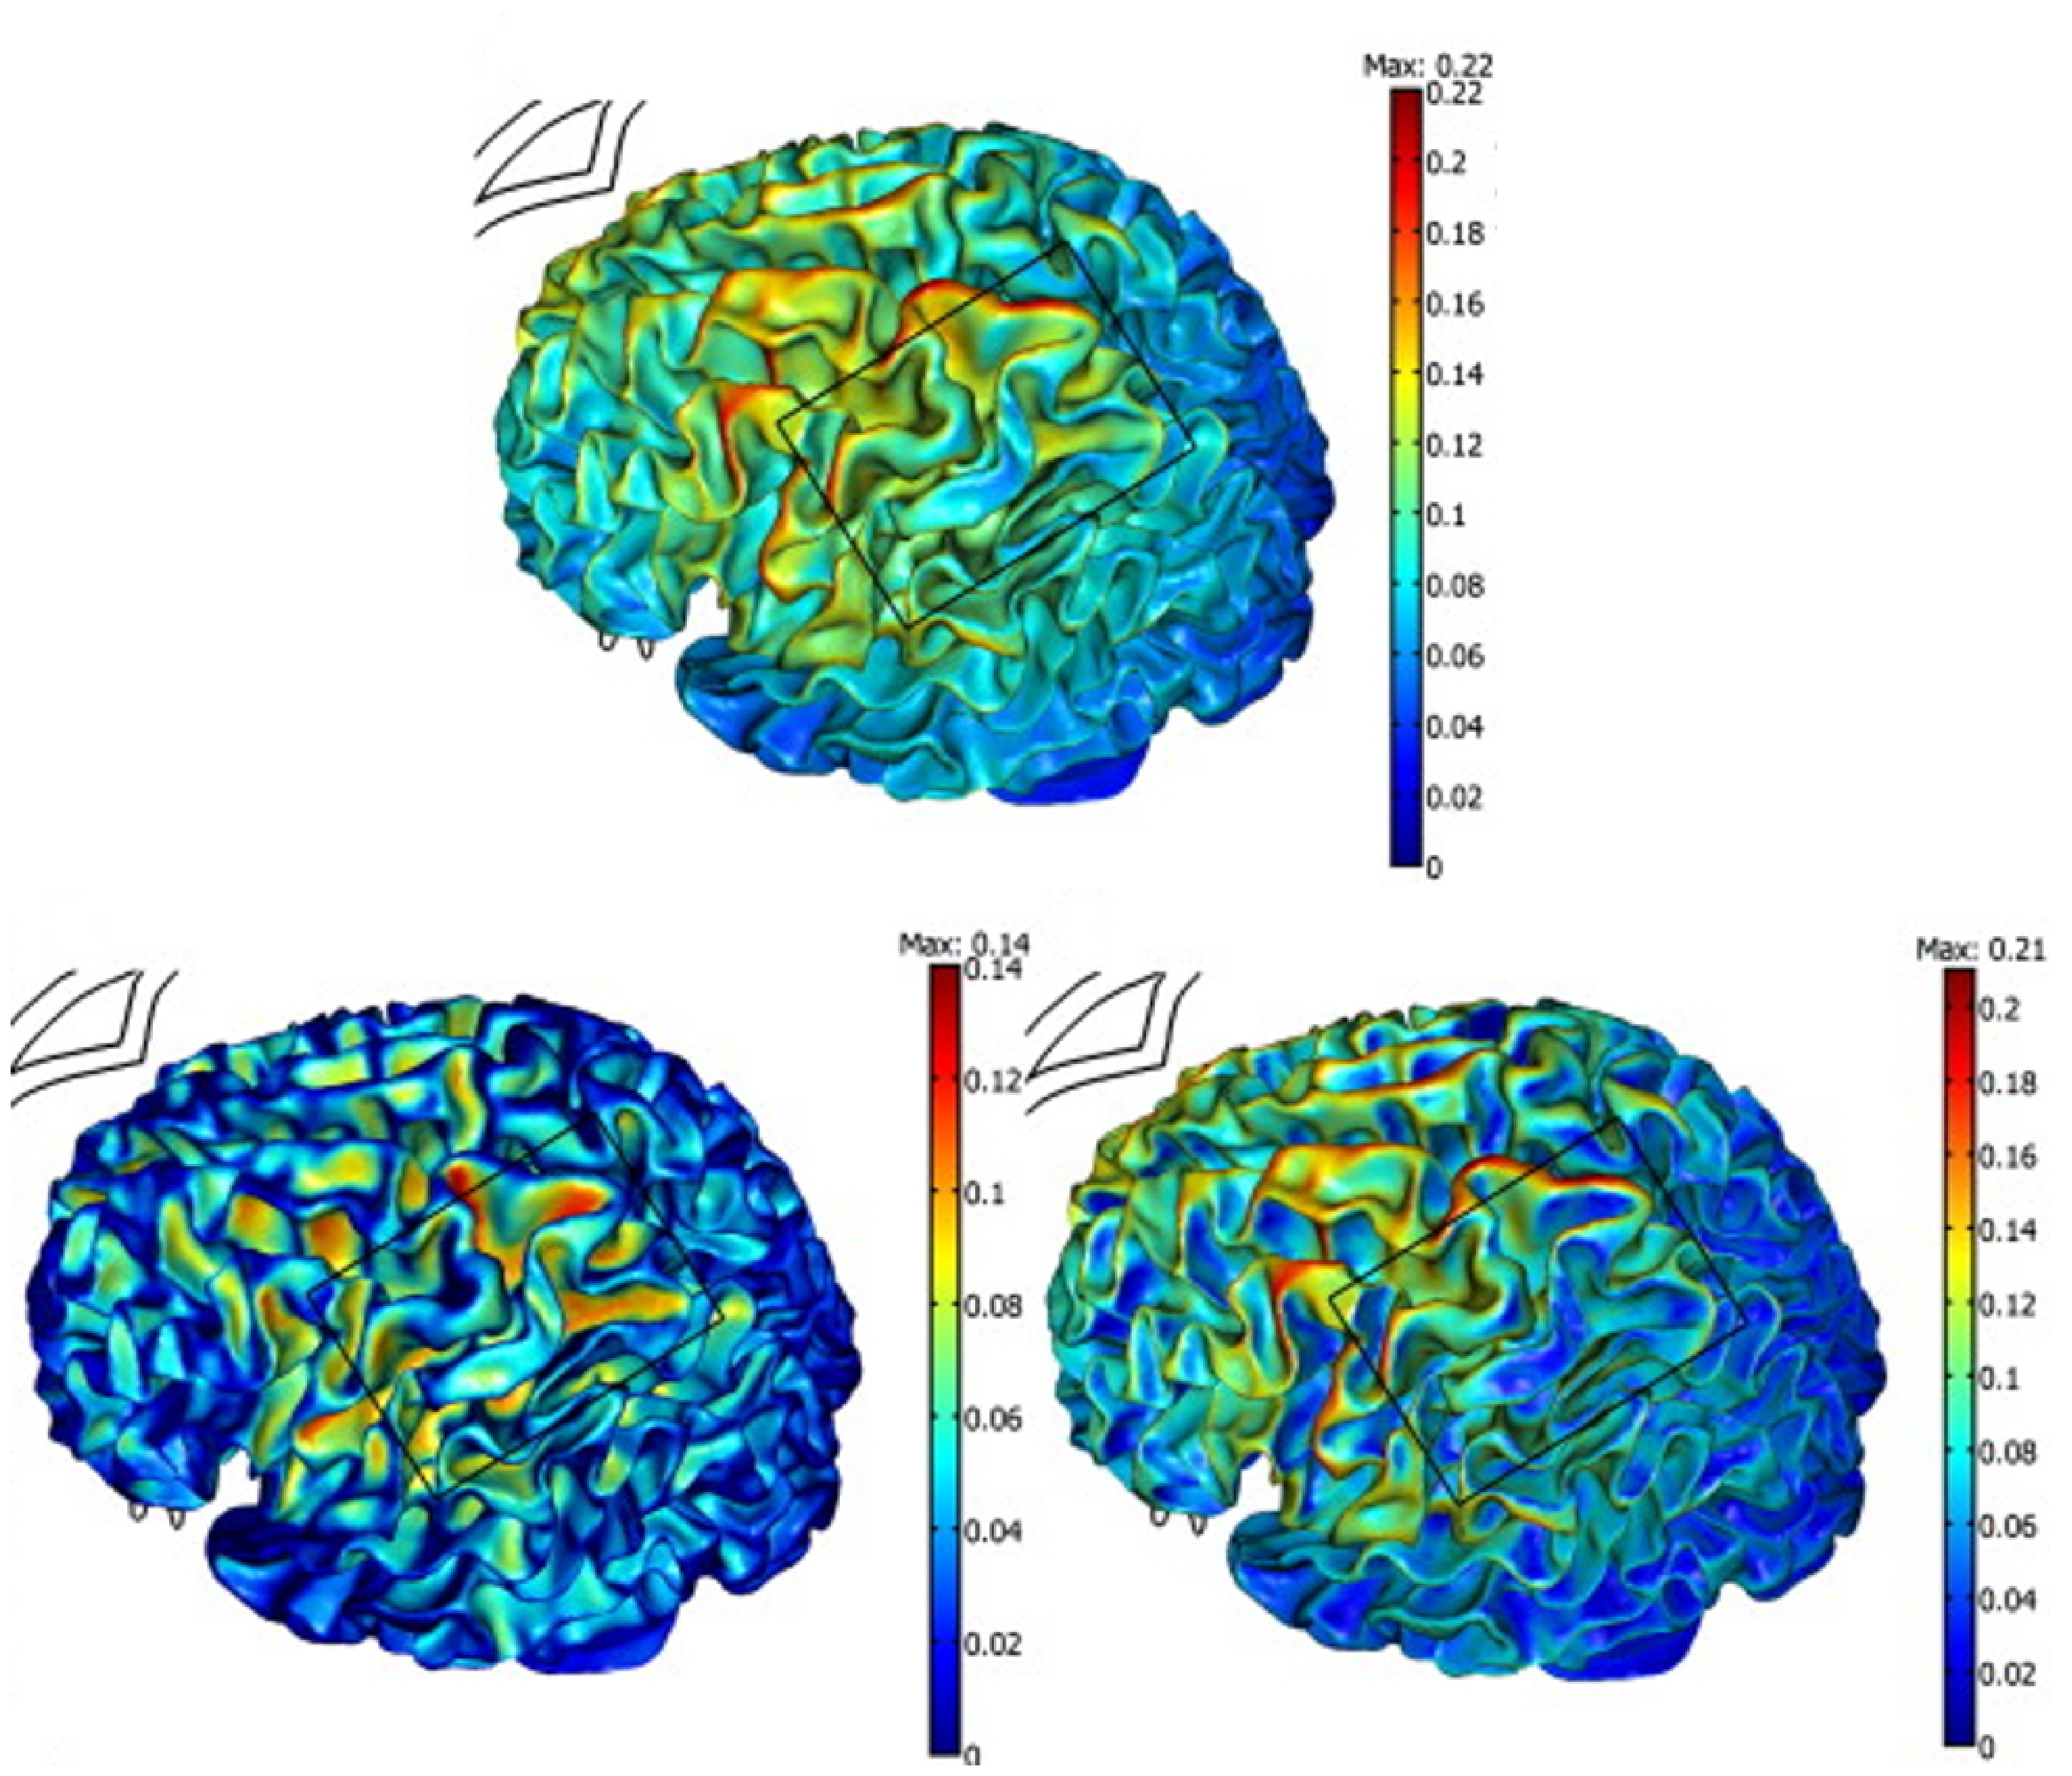
\includegraphics[width = 0.9\textwidth]{electricfields.eps}
\caption{tDCS electric field distributions on the WM surface}
\label{fig:tdcs}
\end{figure}



\subsection{Previous studies}

TDCS Aftereffects

Nitsche and Paulus (2000) discovered exitability changes in motor cortex induced by TDCS. 
They stimulated 10 to 19 subjects with different lengths of DC stimulation and measured MEPs of the 
right abductor digiti minimi when applying TMS during and after stimulation.
The stimulation times varied from 4s up to 5minutes and intensities were between 0.2mA and 1mA. \cite{nitsche00}


In first experiment Nitsche and Paulus measured series 12 TMS-evoked MEPs at the end of 4s long current 
stimulations and without current. 
The same measurements were repeated with different sponge layouts.
They found significant increase and decrease during anodal and cathodal stimulations, respectively. 
The results were, however, found only with sponge layout: other sponge placed on motor cortex and the 
other over the contralateral orbita. 
The other experimets were done with the same sponge layout. \cite{nitsche00}

In other experiment they found differences in MEP sizes after 5 minute DC-stimulation between anodal and 
cathodal stimulation directions. 
The amplitudes were 40$\%$ higher than baseline after anodal stimulation and decreased 30$\%$ in 
comparison to baseline after cathodal stimulation. \cite{nitsche00}


Antal et al. 08: 10Hz AC stimulation over the primary motor cortex showed a trend toward MEP inhibition, when measured after stimulation.

Moliadze et al 10. 140Hz stimulation induces the largest MEP increase. 
Moliadze 12 low 0.2mA intensities resulted in cortical inhibition (increased motor threshold). Intensities between had no effect and 1mA resulted in decreased thresholds witt tACS (Exitatory neurons are less susceptible and require stronger stimulation, but dominate the inhibitory neurons leading to a net effect of excitation.

Nitsche00 our starting point to the research.



\clearpage

\section{Methods}
\subsection{Data}
Data was gathered from 5 different healthy voluntary subjects: 4 males and 1 female. Four of them were righthanded and one was lefthanded. The subjects of age between 23 and 27 years. The measurements were approved by the Ethics Committee of Helsinki University Central Hospital and they followed the principles of the Declaration of Helsinki.


\subsection{Experimental paradigms}

We had two different kind of experimental paradigms for TMS-TES experiments. They both had TES given simultaneously with TMS pulses. In all paradigms subjects motor threshold (MT) was measured either from Abductor pollis brevis (ABP) or from first dorsal interosseus (FDI) muscle of the dominating hand. 

In TES 15 cm$^{2}$ rubber electrodes covered with sponges dipped in salin solution were used. The TES electrodes were placed to be 15 cm from each other measured from the center of the sponge. Electrodes were set on the opposite sides of stimulation point so that electric field would be approximately parrallel to the TMS stimulation direction, see figure \ref{fig:setup}. 

\begin{figure}[here]
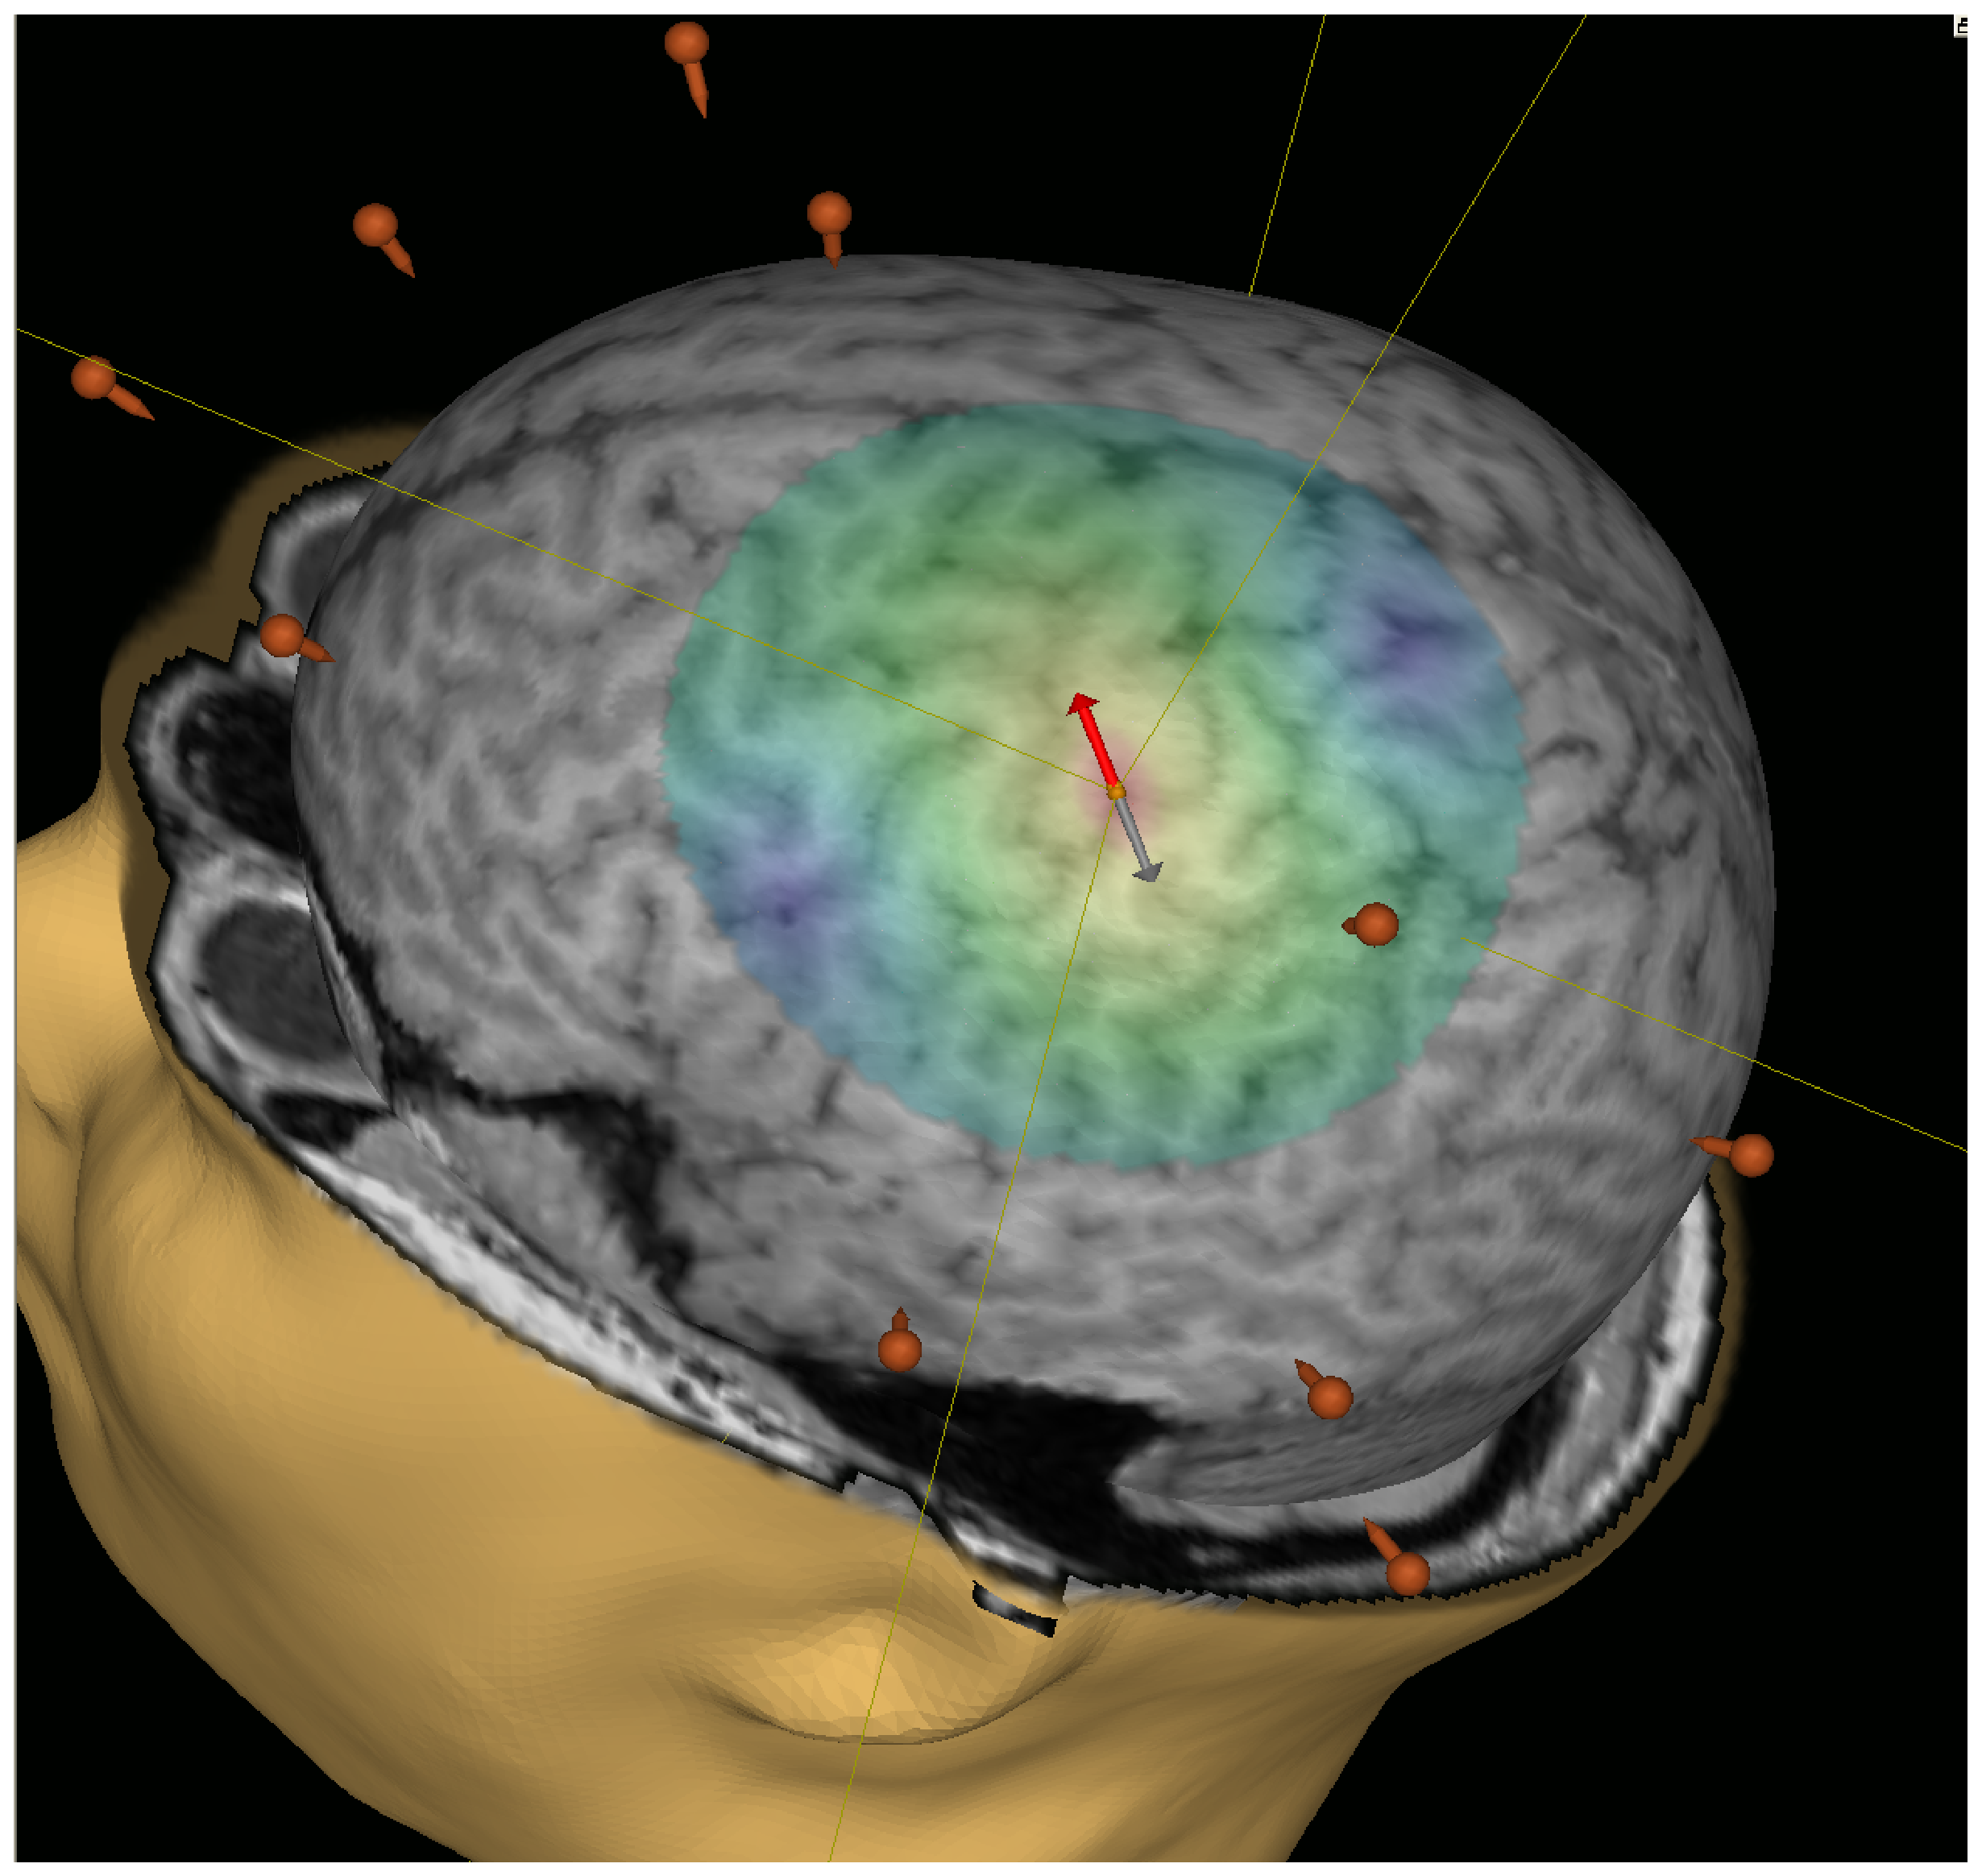
\includegraphics[width = 1.1\textwidth]{subject.eps}
\caption{Stimulation setup}
\label{fig:setup}
\end{figure}

Three subjects underwent an experiment with 9 different stimulation conditions. The conditions differed in current parameter of TDCS stimulation (-2~mV, 0~mV or 2~mV) and in TMS intensity that varied between MT, $MT + 1\%$ and $MT - 1\%$ of stimulator output. The randomized serie of 9 conditions with 50 pulses each was performed twice in so that total of 100 TMS pulses per condition was achived. TMS stimulation was done with monophasic TMS figure-of-eight coil.

Two subject took part in similar experiment, where instead of using different TDCS conditions TACS was used. TACS was set to vary between ?? and ??. Also here the stimulator intensities were set to vary both sides of MT like before. The TMS intensities varied as before with 200 TMS pulses per intensity with monophasic TMS figure-of-eight coil.






\begin{table}[ht!]
  \begin{center}
    \begin{tabular}{c c c c c c c}
    \hline
    Stimulation & Subject & Stimulation & hand  &Coil & Current  & num of \\
     & & target & side &type & type & stimulations \\
    \hline
    1 & Subject1 & FDI & right & monophasic & DC & 900\\
    2 & Subject2 & FDI & right & monophasic & DC & 900\\
    3 & Subject3 & FDI & left  & monophasic & DC & 900\\
    4 & Subject4 & ABP & right & monophasic & AC & 600\\
    5 & Subject5 & ABP & right & monophasic & AC & 600\\
    %6 & Subject1 & ABP & right & biphasic   & DC & 200\\
    %7 & Subject2 & ABP & right & biphasic   & DC & 200\\
    \hline
    \end{tabular}
  \end{center}
  \caption{Stimulation parameters}
\end{table}








\subsection{Data analysis}

Offline analysis was performed with MATLAB (The Mathworks, Inc., Natick,
Massachusetts, USA). First, the data were visually inspected: trials
containing increased EMG baseline activity showing contraction of the target muscle were removed. 




\clearpage
\section{Results}
%\section{Results}




\clearpage
\section{Discussion}
\clearpage
\section{Conclution} 

\clearpage
%% Lähdeluettelo

%% The \phantomsection command is nessesary for hyperref to jump to the 
%% correct page, in other words it puts a hyper marker on the page.

\phantomsection
\addcontentsline{toc}{section}{References}
\bibliography{dippa}{}
\bibliographystyle{plain}
%%\begin{thebibliography}{99}



%%\end{thebibliography}

%% Liitteet
%% Appendices
\clearpage
\appendix
%\phantomsection
%%
%% Lisää tekstin "Liitteet" sisällysluetteloon

%%
%% Adds the word "Appendices" to the table of contents
%\addcontentsline{toc}{section}{Liiteet}
%\addcontentsline{toc}{section}{Appendices}

\section{Appendix example \label{AppendixA}}
%% Liitteiden kaavat, taulukot ja kuvat numeroidaan omana kokonaisuutenaan
%%
%% Equations, tables and figures have their own numbering in Appendices
\renewcommand{\theequation}{A\arabic{equation}}
\setcounter{equation}{0}  
\renewcommand{\thefigure}{A\arabic{figure}}
\setcounter{figure}{0}
\renewcommand{\thetable}{A\arabic{table}}
\setcounter{table}{0}


%% Verbatim-ympäristä ei muotoile tai tavuta tekstiä. Fontti on monospace.
%% Verbatim-ympäristän sisällä annettuja komentoja ei LaTeX käsittele. 
%% Vasta \end{verbatim}-komennon jälkeen jatketaan käsittelyä.
\begin{verbatim}
	\clearpage
	\appendix
	\addcontentsline{toc}{section}{Liite A}
	\section*{Liite A}
	...
	\thispagestyle{empty}
	...
	tekstiä
	...
	\clearpage
\end{verbatim}

Kaavojen numerointi muodostaa liitteissä oman kokonaisuutensa:
\begin{eqnarray}
d \wedge A  &=& F, \label{liitekaava1}\\
d \wedge F  &=& 0. \label{liitekaava2}
\end{eqnarray}


\end{document}
